\documentclass[a4paper, 11pt]{article}
\usepackage{comment} % enables the use of multi-line comments (\ifx \fi) 
\usepackage{fullpage} % changes the margin
\usepackage{amsmath}
\usepackage{graphicx}


\begin{document}


\noindent
\LARGE\textbf{Radius of the Earth} \\
\\
\normalsize \textbf{By: Kevin Dang} \\



\section*{Introduction}

The objective of this experiment was to deduce the radius of the Earth. This was achieved by measuring the variation of gravity using a Sodin gravimeter on different floors of the Burton tower. The height of each floor was also taken into account. In the results section we worked with the full dataset containing all floors, and only floors 3 to 13 as the results for these floors were expected to produce better results, which is explained in the results section. The estimated values for the radius of the Earth were in an acceptable range of error.\\
\\
Some equations relevant to this experiment include: \\

Variation of g on Earth: $\frac{\Delta g}{g} = -2\frac{\Delta R}{R}\Rightarrow R = -2g\frac{\Delta R}{\Delta g}$

Gravitational attraction of the floor: $g' = G\cdot\frac{m_{floor}}{R^2_{to floor}}$

Error propagation for division (and multiplication): $\sigma_z = z\sqrt{(\frac{\sigma_x}{x})^2 + (\frac{\sigma_y}{y})^2}$ 

\section*{Equipment}

\begin{itemize}
\item Sodin gravimeter
\item Gravimeter carrying case
\end{itemize}	


\section*{Experimental Procedure}

\begin{enumerate}
\item Starting from the basement, we placed the gravimeter near the elevators and adjusted the levels properly. We followed the steps in the Radius of the Earth lab guide to do this.
\item After making the final fine adjustment by viewing through the eye-piece, we recorded the counter reading.
\item We repeated this step for all floors and took two datasets so that we have a reference for an uncertainty value in the readings.
\item Later on we estimated the heights of the basement and first floor by counting the number of bricks and measuring each one with a ruler.
\end{enumerate}


\section*{Results}

\subsubsection*{Important values}
\begin{itemize}
\item Gravimeter constant for conversion to mgal: 0.1055
\item Basement Height: 5.10m
\item Floor 1 Height: 5.44m
\item Floors 2-14 Height: 3.95m
\item Mass of each floor (excluding basement and roof): $\approx 10^{6}kg$
\item Gravity in Burton tower Floor 1: g = $9.804253m/s^{2}$
\item Literature value for radius of Earth in Toronto: 6368km
\item Gravimeter reading error: 3 units $\Rightarrow 3\times\frac{0.10055}{1000\times100} = 3.0165\times10^{-6}m/s^2$
\end{itemize}

We chose 3 units as our error for the gravimeter reading since that was the biggest difference between two corresponding values from our two datasets. It accounts for measurement error, human error, and small time difference error. Note that this value must be converted to $m/s^2$ for our calculations.


\subsubsection*{Correcting the reading}
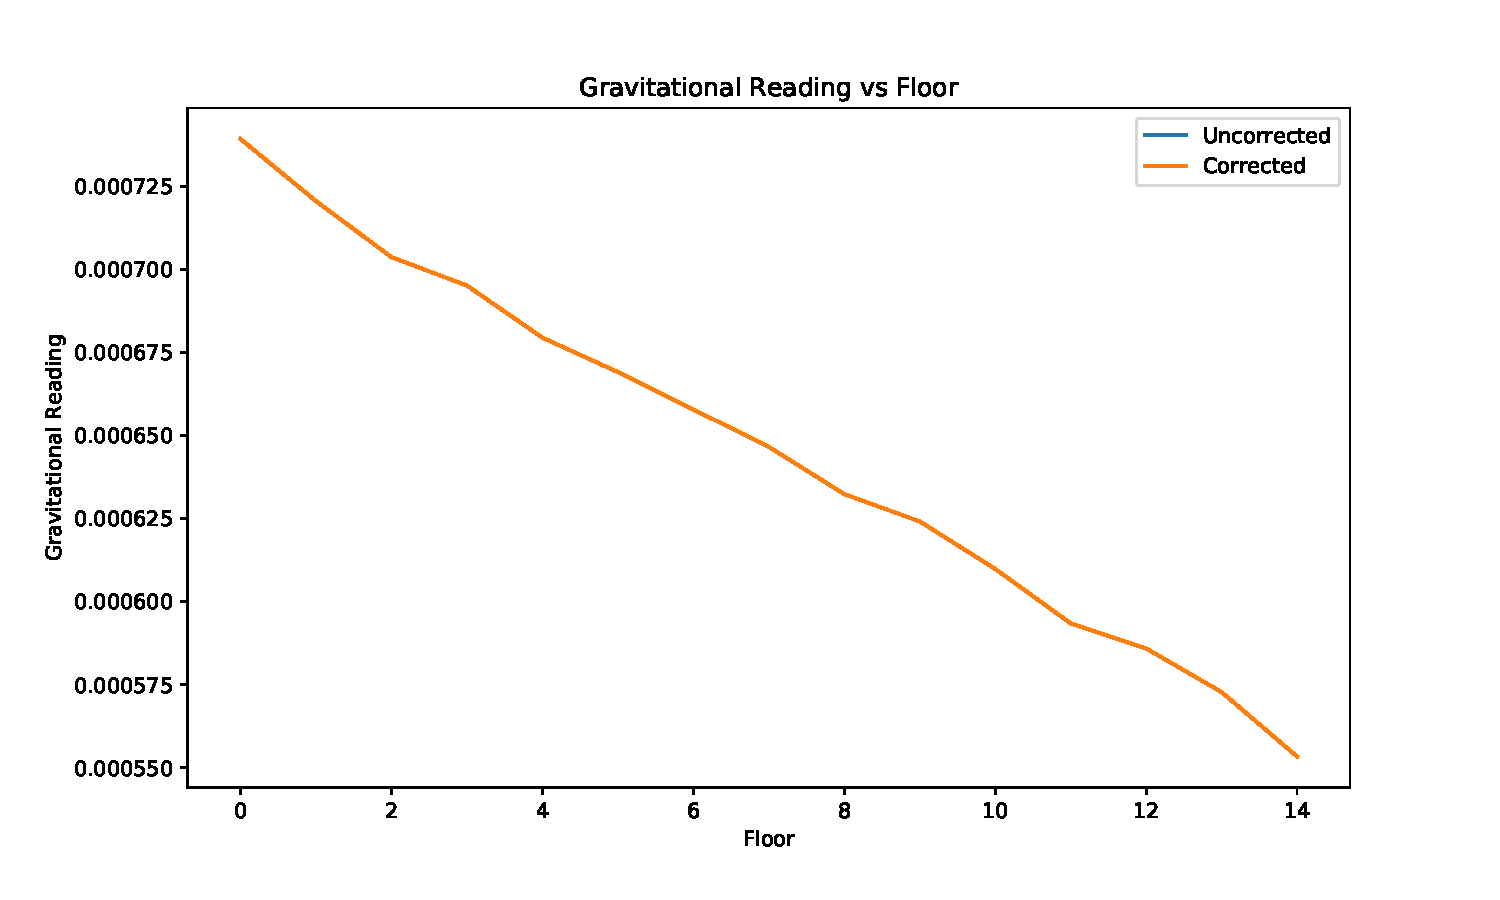
\includegraphics[width=\textwidth]{gravity-floor.pdf}
\\
Since going up each floor will remove mass overhead and put it underneath, we had to correct for this effect in the python file. This was done using the following equation $g' = G\cdot\frac{m_{floor}}{R^2_{to floor}}$ \\
\\
From the above plot we can see that this effect appears to have made very little change to our data. For the purposes of our calculations we used the corrected values.


\subsubsection*{All Floors}
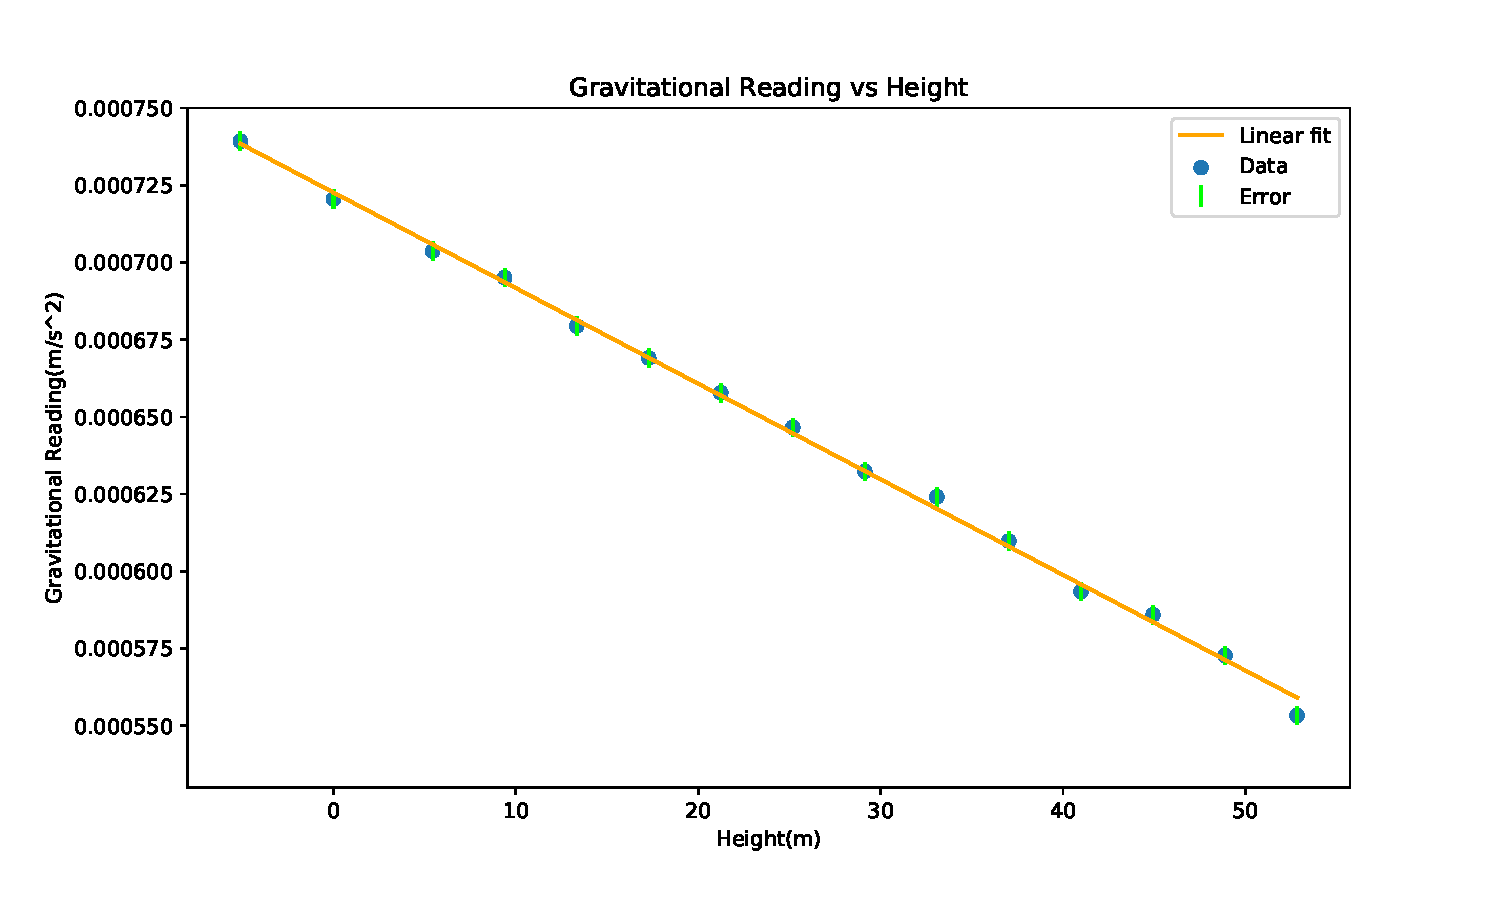
\includegraphics[width=\textwidth]{gravity-height1.pdf}
\\
Equation: $\Delta g = (-3.095\times10^{-6})\Delta R + 722 \times 10^{-6}$
\\
Reduced chi-squared: $\chi^{2}_{red} = 0.7147$ \\
\\
Plotting a graph of $\Delta g$ vs $\Delta R$, we obtain a slope which represents $\frac{\Delta g}{\Delta R}$, so to calculate R, we can use the rearranged first equation from the introduction:

\begin{align*}
R = -2g\frac{\Delta R}{\Delta g} = \frac{-2g}{\frac{\Delta g}{\Delta R}} = \frac{-2(9.804253)}{-3.095\times10^{-6}} = 6335247 \pm 77022m
\end{align*}
\\
The literature value for the radius of the Earth in Toronto is about 6368000m, so our result is smaller by about 32753m or 0.51\%, which is well within our uncertainty range. Note that the uncertainty estimate was obtained in \texttt{Python} by taking the square root of the slope error in the covariance matrix and then using the error propagation formula.

The reduced chi-squared value is a bit low which suggests potential overfitting to the data. This is not surprising considering the fact that there are only 15 data points. The goodness of fit is not great but we obtained acceptable results. In the next section we work with floors 3 to 13 so there will be even fewer data points!

\subsubsection*{Floors 3 to 13}
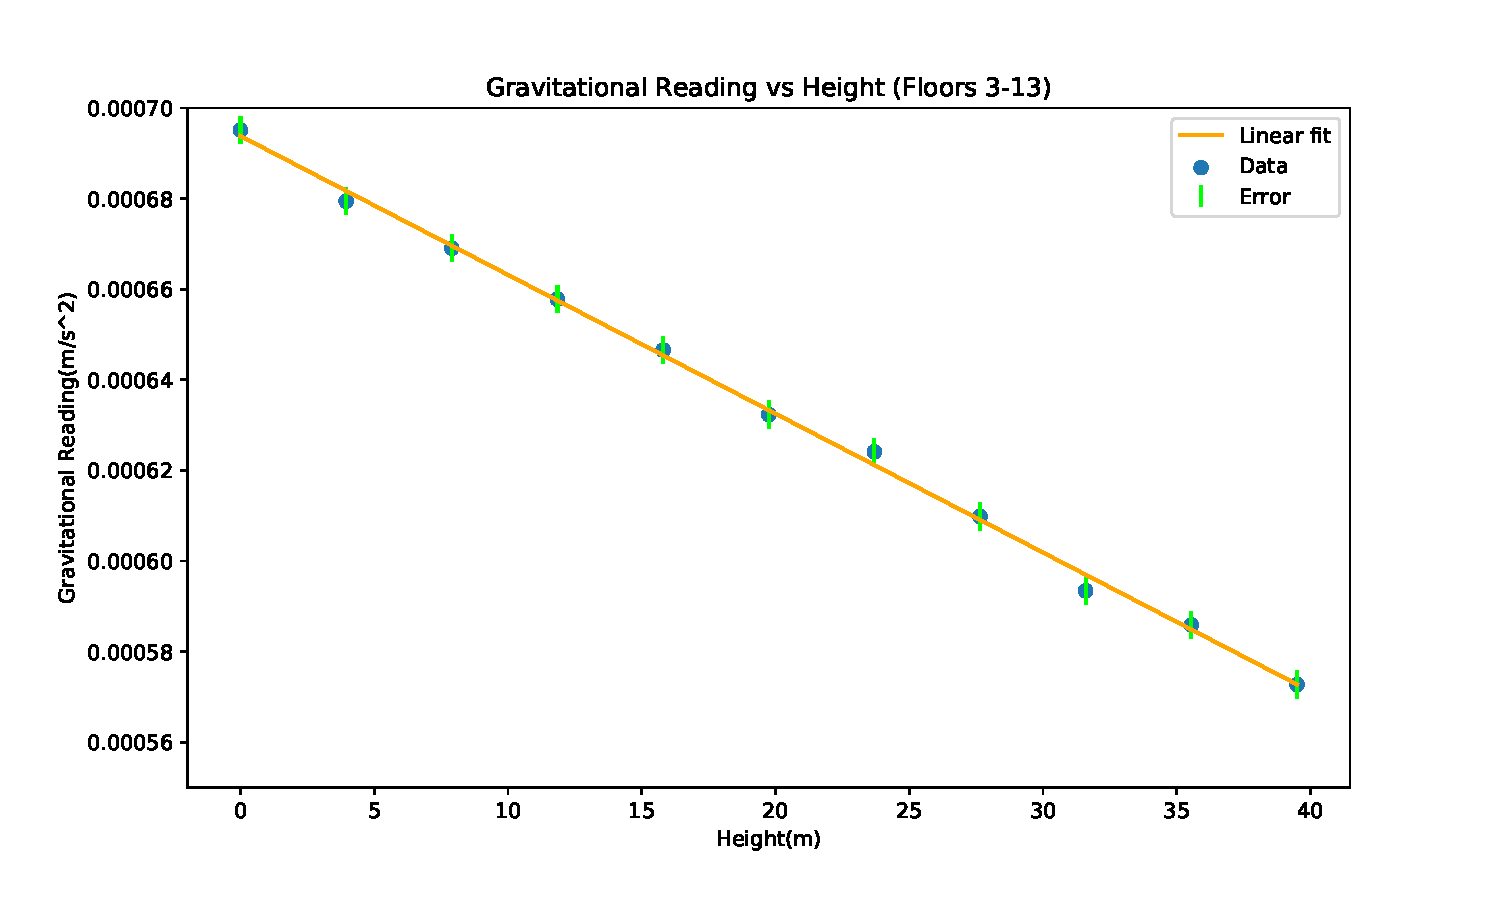
\includegraphics[width=\textwidth]{gravity-height2.pdf}
\\
Equation: $\Delta g = (-3.065\times10^{-6})\Delta R + 694 \times 10^{-6}$
\\
Reduced chi-squared: $\chi^{2}_{red} = 0.394$ \\
\\
Plotting a graph of $\Delta g$ vs $\Delta R$, we obtain a slope which represents $\frac{\Delta g}{\Delta R}$, so to calculate R, we can use the rearranged first equation from the introduction:

\begin{align*}
R = -2g\frac{\Delta R}{\Delta g} = \frac{-2g}{\frac{\Delta g}{\Delta R}} = \frac{-2(9.804253)}{-3.065\times10^{-6}} = 6398340 \pm 95468m
\end{align*}
\\
The literature value for the radius of the Earth in Toronto is about 6368000m, so our result is larger by about 30340m or 0.48\%, which is well within our uncertainty range. Note that the uncertainty estimate was obtained in \texttt{Python} by taking the square root of the slope error in the covariance matrix and then using the error propagation formula.

The reduced chi-squared is quite low, which is due to the small number of data points used in the model. Although the goodness of fit is not as good as the previous model containing data points for every floor, the estimated value for the radius of the Earth obtained with this model is more accurate. This is likely due to the fact that the basement (floor 0) is a missing mass, and the heights of the basement and first floor are not standard so we were required to estimate the heights by counting bricks and measuring with a ruler, which is not very accurate. The fourteenth floor was also excluded since it only had the roof above it, and the mass of the roof is smaller than the mass of the floors.

\section*{Questions}
\subsubsection*{Question 1}
\textit{"The linear portion of your graph should be able to provide data that will give R to about 1\% or 2\%. However, also of interest is the deviation from linearity near the basement or the fifteenth floor. What does this deviation tell you? At what level would the centrifugal force due to the earth's rotation affect the result of this experiment? How important is the earth's eccentricity?"} \\
\\
This deviations tells us that ours results were affected by different heights and masses near the basement and near the upper floors. Our assumption is probably correct, and as shown in our results, using floors 3 to 13 yielded a more accurate estimate of the Earth's radius compared to using the whole dataset. \\
\\
The centrifugal force due to the Earth's rotation would affect the result of this experiment at the basement. This is a result of the equation: $F = m\omega^2r$. A smaller height means that the angular velocity will be significantly larger due to its squared term. \\
\\
The Earth's eccentricity determines how close the Earth is to the sun at a certain time in the year. The eccentricity does not change much over a short period of time, so it does not have a significant impact on the results of this experiment.


\subsubsection*{Question 2}
\textit{"The Greek Genius, Eratosthenes, obtained the radius of the earth to $\sim\pm80km$ in 200 BC for the cost of a trip to Upper Egypt. How does this compare with the cost of a \$16k gravity meter?"} \\
\\
The estimated radius from our experiment using floors 3 to 13 is larger by about 30km, which is more accurate than what  Eratosthenes obtained. This is not surprising since the gravity meter costs significantly more than a trip to Upper Egypt, though it is quite impressive that Eratosthenes was able to obtain a good estimate of the Earth's radius.

\section*{Conclusion}
Our second model gave an estimate for the radius of the Earth of about 6398km using the gravimeter was within about 30km or 0.48\% of the literature value of 6368km. This result was obtained using only floors 3 to 13, which represented our "best" data since there was an issue with different heights and masses at certain floors, which were excluded from the model. The goodness of fit was not great since we had few data points, but the result turned out to be acceptable. The first model which included all floors yielded an acceptable result which had an error 0.51\% and a decent goodness of fit compared to our second model since it had more data points, but it was not quite as accurate as our second model due to the reasons mentioned above.


\end{document}
